%%%%%%%%%%%%%%%%%%%%%%%%%%%%%%%%%%%%%%%%%
% Beamer Presentation
% LaTeX Template
% Version 1.0 (10/11/12)
%
% This template has been downloaded from:
% http://www.LaTeXTemplates.com
%
% License:
% CC BY-NC-SA 3.0 (http://creativecommons.org/licenses/by-nc-sa/3.0/)
%
%%%%%%%%%%%%%%%%%%%%%%%%%%%%%%%%%%%%%%%%%

%----------------------------------------------------------------------------------------
%	PACKAGES AND THEMES
%----------------------------------------------------------------------------------------

\documentclass[dvipsnames]{beamer}
%\usepackage[lighttt]{lmodern}
\usepackage{lmodern}
%\usepackage{luximono}
\usepackage{xcolor}
%\renewcommand{\ttdefault}{pcr}
\usepackage{listings}
\mode<presentation> {

% The Beamer class comes with a number of default slide themes
% which change the colors and layouts of slides. Below this is a list
% of all the themes, uncomment each in turn to see what they look like.

%\usetheme{default}
%\usetheme{AnnArbor}
%\usetheme{Antibes}
%\usetheme{Bergen}
%\usetheme{Berkeley}
%\usetheme{Berlin}
%\usetheme{Boadilla}
%\usetheme{CambridgeUS}
%\usetheme{Copenhagen}
%\usetheme{Darmstadt}
%\usetheme{Dresden}
%\usetheme{Frankfurt}
%\usetheme{Goettingen}
%\usetheme{Hannover}
%\usetheme{Ilmenau}
%\usetheme{JuanLesPins}
%\usetheme{Luebeck}
\usetheme{Madrid}
%\usetheme{Malmoe}
%\usetheme{Marburg}
%\usetheme{Montpellier}
%\usetheme{PaloAlto}
%\usetheme{Pittsburgh}
%\usetheme{Rochester}
%\usetheme{Singapore}
%\usetheme{Szeged}
%\usetheme{Warsaw}

% As well as themes, the Beamer class has a number of color themes
% for any slide theme. Uncomment each of these in turn to see how it
% changes the colors of your current slide theme.

%\usecolortheme{albatross}
%\usecolortheme{beaver}
%\usecolortheme{beetle}
%\usecolortheme{crane}
%\usecolortheme{dolphin}
%\usecolortheme{dove}
%\usecolortheme{fly}
%\usecolortheme{lily}
%\usecolortheme{orchid}
%\usecolortheme{rose}
%\usecolortheme{seagull}
%\usecolortheme{seahorse}
%\usecolortheme{whale}
%\usecolortheme{wolverine}

%\setbeamertemplate{footline} % To remove the footer line in all slides uncomment this line
%\setbeamertemplate{footline}[page number] % To replace the footer line in all slides with a simple slide count uncomment this line

%\setbeamertemplate{navigation symbols}{} % To remove the navigation symbols from the bottom of all slides uncomment this line
}

\usepackage{graphicx} % Allows including images
%\usepackage{booktabs} % Allows the use of \toprule, \midrule and \bottomrule in tables

\lstdefinestyle{mypython}{
breaklines=true,
basicstyle=\scriptsize\ttfamily,
showstringspaces=false,
keywordstyle=\bfseries\color{green!40!black},
commentstyle=\itshape\color{purple!40!black},
identifierstyle=\color{black},%\color{blue},
stringstyle=\color{orange}
}
\lstset{escapechar=€,style=mypython}
\setbeamertemplate{navigation symbols}{}
%----------------------------------------------------------------------------------------
%	TITLE PAGE
%----------------------------------------------------------------------------------------

\title[httk and omdb]{What are the \emph{httk} and the \emph{omdb}?\\And, what can they do for YOU?} 

\author{Rickard Armiento} % Your name
\institute[LiU]{Link{\"o}ping University, Sweden} % Your institution as it will appear on the bottom of every slide, may be shorthand to save space
%{
%Link{\"o}ping University \\ % Your institution for the title page
%\medskip
%\textit{john@smith.com} % Your email address
%}
%\date{\today} % Date, can be changed to a custom date

%\let\oldframe\frame
%\renewcommand{\frame}{%
%\oldframe
%\let\olditemize\itemize
%\renewcommand\itemize{\olditemize\addtolength{\itemsep}{10pt}}%
%}
\titlegraphic{\strut\\[0.8cm]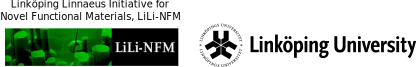
\includegraphics[width=\linewidth]{logos.pdf}}
\begin{document}

\begin{frame}
\titlepage 
\end{frame}

\section{Overview}
\begin{frame}
\frametitle{Overview}
{\color{blue} The High-Throughput Toolkit (\emph{httk})}
\begin{itemize}
\item A toolkit for {\color{red}preparing} and {\color{red}running} calculations, {\color{red}analyzing} the result,  {\color{red}store them in a global and/or in a personalized database.}
\item The primary focus is {\color{red} automatization:} run with as little human intervention as possible.
\item \emph{Crucial} for large datasets; \emph{convenient} for smaller projects!
\item Intended to expand beyond atomistic calculations, but those are our primary focus for now.
\end{itemize}\strut\\[0.2cm]

{\color{blue}The Open Materials Database (omdb)}
\begin{itemize}
\item A central collection of computational data where we store our results.
\item You can, if you want, submit results there as well.
\item Easily interacts with \emph{httk}; built using \emph{httk}.
\end{itemize}
\end{frame}

\begin{frame}
\frametitle{Database-centric High-Throughput}
The \emph{httk} is an independent implementation of the Database-centric high-throughput methodology pioneered by G.\ Ceder, and others.\\[0.2cm]
{\scriptsize\centering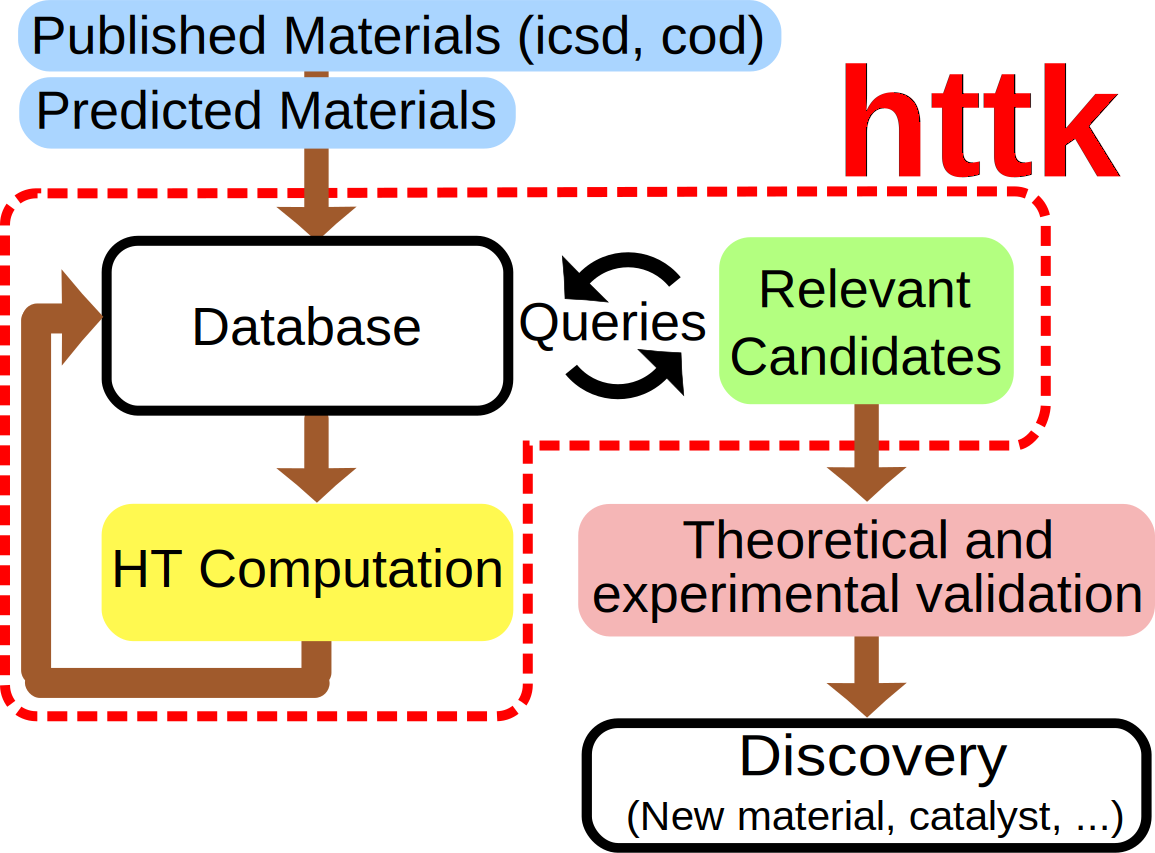
\includegraphics[width=0.6\linewidth]{flowchart_databasedriven_ht.pdf}\\[0.5cm]}

\raggedright See: A. Jain, G. Hautier, C. J. Moore, S. P. Ong, C. C. Fischer, T. Mueller, K. A. Persson, G. Ceder, Comp. Mat. Sci. \textbf{50}, 2295 (2011).\\
\end{frame}

\begin{frame}
\frametitle{Overview}
Components:\\[0.1cm]
\begin{itemize}
\item The \emph{httk} python library:
\begin{itemize}
  \item Handling crystal structures.
  \item Prepare calculations to be run.
  \item Storage, retrieval, search and analysis of data in database.
\end{itemize}
\vspace{0.5cm}
\item The \emph{httk} scripts:
\begin{itemize}
  \item Handling large sets of computer runs.
  \item Scripting that allow advanced multi-stage runs to be run on clusters with limited walltime.
  \item Managing ongoing runs across many supercomputers.
  \item Easy submission of results to \emph{omdb}. 
\end{itemize}
\end{itemize}
\end{frame}

\begin{frame}
\frametitle{Overview}
Why not extend existing libraries (ASE, pymatgen, etc.) instead?\\[0.1cm]
\begin{itemize}
  \item Different core design choices
  \begin{itemize}
    \item {\color{red}Database interaction as easy as possible;} python objects can be stored, searched, retrieved; mixing different databases.
    \item Preserves numbers exactly (fractions instead of floating point), helps a lot with crystal geometry and database interaction.
  \end{itemize}
  \item Different attitude to dependencies
  \begin{itemize}  
    \item {\color{red}No libraries outside standard python needed to get \emph{httk} up and running.} Not even numpy or scipy.
    \item Other libraries can be/are called when needed.
    \item \emph{httk} goes out of its way to help you load the library you want from e.g. odd locations (helpful to, e.g., avoid old system-wide version)
  \end{itemize}
  \item Instead, \emph{httk} is compatible / interacts with those libraries; i.e., you {\color{red}can translate between ASE, pymatgen, etc.,} and use their features interchangeably.
\end{itemize}
%\scriptsize (Also: more protective license; code stays free, your contributions not 'taken' into closed source.)
\end{frame}

\section{Examples}
\begin{frame}
\frametitle{Examples}
A few programming examples for atomistic computation will follow.\\
\strut\\
(This is a more technical part of this presentation)
\end{frame}

%%%%%%%%%%%%%%%%%%%%%%%%%%%%%%%%%%%%%%%%%%%############################

\defverbatim[colored]\inputone{
\begin{lstlisting}[language=python,style=mypython,frame=single]
import httk

struct = httk.load("example.cif")

print("Formula:", struct.formula)
print("Volume", float(struct.uc_volume))
print("Assignments", struct.uc_formula_symbols)
print("Counts:", struct.uc_counts)
print("Coords", struct.uc_reduced_coords)
\end{lstlisting}
}

\defverbatim[colored]\outputone{
\begin{lstlisting}[language=python,style=mypython,frame=single]
('Formula:', 'BO2Tl')
('Volume', 509.24213999999984)
('Assignments', ['B', 'O', 'Tl'])
('Counts:', [8, 16, 8])
('Coords', FracVector(((1350, 4550, 4250), ..., ,10000)))
\end{lstlisting}
}

%\begin{lstlisting}
%import httk

%struct = httk.load("example.cif")

%print("Formula:", struct.formula)
%print("Volume", float(struct.uc_volume))
%print("Assignments", struct.uc_symbols)
%print("Counts:", struct.uc_counts)
%print("Coords", struct.uc_reduced_coords)
%\end{lstlisting}

\begin{frame}
\frametitle{Examples: Structures}
Very easy to load a cif file, or poscar, etc.:
\inputone
Output:
\outputone
\end{frame}

%%%%%%%%%%%%%%%%%%%%%%%%%%%%%%%%%%%%%%%%%%%%%%%%%%%%%%%%%%%%%%%%%%%%%%%%%

\defverbatim[colored]\inputone{
\begin{lstlisting}[language=python,style=mypython,frame=single]
from httk.atomistic import Structure

cell = [[1.0, 0.0, 0.0],
        [0.0, 1.0, 0.0],
        [0.0, 0.0, 1.0]]

coordgroups = [[
                 [0.5, 0.5, 0.5] 
               ],[
                 [0.0, 0.0, 0.0] 
               ],[
                 [0.5, 0.0, 0.0],[0.0, 0.5, 0.0],[0.0, 0.0, 0.5]
              ]]

assignments = ['Pb','Ti','O']
volume=62.79
struct = Structure.create(uc_cell=cell,
            uc_reduced_coordgroups=coordgroups,
            assignments=assignments,
            uc_volume=volume)

\end{lstlisting}
}

\begin{frame}
\frametitle{Examples: Structure}
Of course one can also create and modify structures directly in code:
\inputone
\end{frame}

%%%%%%%%%%%%%%%%%%%%%%%%%%%%%%%%%%%%%%%%%%%%%%%%%%%%%%%%%%%%%%%%%%%%%%%%

\defverbatim[colored]\inputone{
\begin{lstlisting}[language=python,style=mypython,frame=single]
import httk
import httk.atomistic.vis

struct = httk.load("POSCAR")
struct.vis.show()
\end{lstlisting}
}

\begin{frame}
\frametitle{Examples: Visualization}
Easy visualization using, e.g., jmol
\inputone
\includegraphics[width=8cm]{httk_unitcell.jpg}
\end{frame}

%%%%%%%%%%%%%%%%%%%%%%%%%%%%%%%%%%%%%%%%%%%%%%%%%%%%%%%%%%%%%%%%%%%%%%%%%%

%\defverbatim[colored]\inputone{
%\begin{lstlisting}[language=python,style=mypython,frame=single]
%import httk

%struct = httk.load("POSCAR")

%print("Formula:", struct.formula)
%hall_symbol = struct.hall_symbol
%spacegroup_number = struct.spacegroup_number
%print("Spacegroup info:",hall_symbol, spacegroup_number)
%\end{lstlisting}
%}

%\defverbatim[colored]\outputone{
%\begin{lstlisting}[language=python,style=mypython,frame=single]
%('Formula:', 'O3PbTi')
%('Spacegroup info', '-P 4 2 3', 221)
%\end{lstlisting}
%}

%\begin{frame}
%\frametitle{Examples: Structure}
%Find symmetry information (calls out to ISOTROPY software):
%\inputone
%Output:
%\outputone
%\end{frame}

%\defverbatim[colored]\inputone{
%\begin{lstlisting}[language=python,style=mypython,frame=single]
%import httk
%
%struct = httk.load("POSCAR")
%
%print("Formula:", struct.formula)
%hall_symbol = struct.hall_symbol
%spacegroup_number = struct.spacegroup_number
%print("Spacegroup info:",hall_symbol, spacegroup_number)
%\end{lstlisting}
%}

%%%%%%%%%%%%%%%%%%%%%%%%%%%%%%%%%%%%%%%%%%%%%%%%%%%%%%%%%%%%%%

\defverbatim[colored]\inputone{
\begin{lstlisting}[language=python,style=mypython,frame=single]
from httk.atomistic import Structure
import httk.atomistic.vis
import httk.external.ase_glue
import ase.lattice.surface

slab = ase.lattice.surface.fcc111('Al', size=(2,2,10), vacuum=10.0)
struct = Structure.ase.from_Atoms(slab)
struct.vis.show()
\end{lstlisting}
}

\begin{frame}
\frametitle{Examples: External libraries}
Easy interaction with other useful libraries and software, e.g., ASE:\tiny\\
(Present bindings: ASE, aflow, cif2cell, isotropy, jmol, pymatgen, platon, gulp)
\inputone
\includegraphics[width=8cm]{httk_slab.jpg}
\end{frame}

%%%%%%%%%%%%%%%%%%%%%%%%%%%%%%%%%%%%%%%%%%%%%%%%%%%%%%%%%%%%%%%%

\defverbatim[colored]\inputone{
\begin{lstlisting}[language=python,style=mypython,frame=single]
import httk
import httk.atomistic.vis

struct = httk.load("POSCAR")
supercell1 = struct.build_supercell([[2,0,0],[0,2,0],[0,0,1]])
supercell1.vis.show()
supercell2 = struct.build_orthogonal_supercell(tolerance=20)
supercell2.vis.show()
supercell3 = struct.build_cubic_supercell(tolerance=20)
supercell3.vis.show()
\end{lstlisting}
}

\begin{frame}
\frametitle{Examples: Supercells}
Build supercells, find orthogonal and cubic ones:
\inputone
\includegraphics[width=6cm]{httk_ortho.jpg}
\includegraphics[width=6cm]{httk_cubic.jpg}
\end{frame}

%%%%%%%%%%%%%%%%%%%%%%%%%%%%%%%%%%%%%%%%%%%%%%%%%%%%%%%%%%%%%%%%%
\defverbatim[colored]\inputone{
\begin{lstlisting}[language=python,style=mypython,frame=single]
import httk
import httk.db

backend = httk.db.backend.Sqlite('example.sqlite')
store = httk.db.store.SqlStore(backend)

struct = httk.load('example.cif')
store.save(struct)
\end{lstlisting}
}

\defverbatim[colored]\inputtwo{
\begin{lstlisting}[language=bash,style=mypython,frame=single]
user@computer:> sqlitebrowser example.sqlite
\end{lstlisting}
}

\begin{frame}
\frametitle{Examples: Database}
Store data in a local relational database (sqlite):
\inputone
\inputtwo
\includegraphics[width=6cm]{database.png}
\end{frame}

%%%%%%%%%%%%%%%%%%%%%%%%%%%%%%%%%%%%%%%%%%%%%%%%%%%%%%%%%%%%%

\defverbatim[colored]\inputone{
\begin{lstlisting}[language=python,style=mypython,frame=single]
import httk
from httk.atomistic import Structure
import httk.db

backend = httk.db.backend.Sqlite('example.sqlite')
store = httk.db.store.SqlStore(backend)

search = store.searcher()
search_struct = search.variable(Structure)
search.add( search_struct.uc_nbr_atoms < 40 )

search.output(search_struct,'structure')

for match, header in search:
    struct = match[0]
    print("Found:",struct.formula)
\end{lstlisting}
}

\defverbatim[colored]\outputone{
\begin{lstlisting}[language=python,style=mypython,frame=single]
('Found:','ZnO2')
\end{lstlisting}
}

\begin{frame}
\frametitle{Examples: Database}
Search in your local database:
\inputone
Output:
\outputone
\end{frame}

\defverbatim[colored]\inputtwo{
\begin{lstlisting}[language=bash,style=mypython,frame=single]
user@computer:> cd Run
user@computer:> vasp
\end{lstlisting}
}

\defverbatim[colored]\outputone{
\begin{lstlisting}[language=bash,style=mypython,frame=single]
 running on    1 nodes
 distr:  one band on    1 nodes,    1 groups
 vasp.5.2.12 11Nov11 complex                                                    
  
 POSCAR found type information on POSCAR  Ti N 
 POSCAR found :  2 types and       2 ions

 ----------------------------------------------------------------------------- 
|                                                                             |
|  ADVICE TO THIS USER RUNNING 'VASP/VAMP'   (HEAR YOUR MASTER'S VOICE ...):  |
|                                                                             |
|      You have a (more or less) 'small supercell' and for smaller cells      |
|      it is recommended  to use the reciprocal-space projection scheme!      |
\end{lstlisting}
}

%%%%%%%%%%%%%%%%%%%%%%%%%%%%%%%%%%%%%%%%%%%%%%%%%%%

\defverbatim[colored]\inputone{
\begin{lstlisting}[language=python,style=mypython,frame=single]
import httk
import httk.iface.vasp_if

poscarspath="/path/to/your/poscars/POT_GGA_PAW_PBE/"

struct = httk.load("example.cif")

httk.iface.vasp_if.prepare_single_run("Run", struct, 
     template='t:vasp/single/static', poscarspath=poscarspath)
\end{lstlisting}
}

\begin{frame}
\frametitle{Examples: Computations}
Setup a simple VASP calculation to run manually:
\inputone
\inputtwo
Output:
\outputone
\end{frame}

%%%%%%%%%%%%%%%%%%%%%%%%%%%%%%%%%%%%%%%%%%%%%%%%%%%

\defverbatim[colored]\inputone{
\begin{lstlisting}[language=python,style=mypython,frame=single]
import httk, httk.task, httk.db
from httk.atomistic import Structure

backend = httk.db.backend.Sqlite('tutorial.sqlite')
store = httk.db.store.SqlStore(backend)

search = store.searcher()
search_struct = search.variable(Structure)
search.add_all(search_struct.formula_symbols.is_in('O','Ca','Ti'))
search.output(search_struct,'structure')

for match, header in search:
  struct = match[0]
  httk.task.create_batch_task('Runs','/vasp/batch/relax',
    {"structure":struct})
\end{lstlisting}
}

\begin{frame}
\frametitle{Examples: Computations}
Generate a big batch of computations:
\inputone
\end{frame}

%%%%%%%%%%%%%%%%%%%%%%%%%%%%%%%%%%%%%%%%%%%%%%%%%%%

\defverbatim[colored]\inputone{
\begin{lstlisting}[language=bash,style=mypython,frame=single]
user@computer:> httk-project-setup example_project
user@computer:> httk-computer-setup ssh-slurm kappa 
user@computer:> httk-computer-install kappa
\end{lstlisting}
}

\defverbatim[colored]\inputtwo{
\begin{lstlisting}[language=bash,style=mypython,frame=single]
user@computer:> httk-tasks-send-to-computer kappa Runs/
user@computer:> httk-tasks-start-taskmanager kappa
\end{lstlisting}
}

\defverbatim[colored]\inputthree{
\begin{lstlisting}[language=bash,style=mypython,frame=single]
user@computer:> httk-tasks-status kappa 
\end{lstlisting}
}

\defverbatim[colored]\inputfour{
\begin{lstlisting}[language=bash,style=mypython,frame=single]
user@computer:> httk-tasks-receive-from-computer kappa Runs/
\end{lstlisting}
}

\begin{frame}
\frametitle{Examples: Computations}
Run the batch of computations on a supercomputer ('kappa'):
\inputone
\inputtwo
\inputthree
\inputfour
\end{frame}

%%%%%%%%%%%%%%%%%%%%%%%%%%%%%%%%%%%%%%%%%%%%%%%%%%%
\defverbatim[colored]\inputone{
\begin{lstlisting}[language=python,style=mypython,frame=single]
import httk, httk.db, httk.task, os
from httk.atomistic.results import Result_TotalEnergyResult

backend = httk.db.backend.Sqlite('example.sqlite')
store = httk.db.store.SqlStore(backend)

reader = httk.task.reader('./','Runs/')

for rundir, computation in reader:
    struct = httk.load(os.path.join(rundir,"CONTCAR"))
    outcar = httk.iface.vasp_if.read_outcar(os.path.join(rundir,"OUTCAR.cleaned.relax2"))            
    total_energy_result = Result_TotalEnergyResult(computation, struct, float(outcar.final_energy))
    store.save(total_energy_result) 

\end{lstlisting}
}

\begin{frame}
\frametitle{Examples: Computations}
Read results back into database
\inputone
\end{frame}

%%%%%%%%%%%%%%%%%%%%%%%%%%%%%%%%%%%%%%%%%%%%%%%%%%%

\defverbatim[colored]\inputone{
\begin{lstlisting}[language=python,style=mypython,frame=single]
import httk, httk.db, httk.task, httk.atomistic.vis
from httk.atomistic import Structure, StructurePhaseDiagram 
from httk.atomistic.results import Result_TotalEnergyResult

backend = httk.db.backend.Sqlite('example.sqlite')
store = httk.db.store.SqlStore(backend)
search = store.searcher()
search_total_energy = search.variable(Result_TotalEnergyResult)
search_struct = search.variable(Structure)
search.add(search_total_energy.structure == search_struct)
search.add_all(search_struct.formula_symbols.is_in('O','Ca','Ti'))
search.output(search_total_energy,'total_energy_result')

structures, energies = [],[]
for match, header in search:
    total_energy_result = match[0]
    structures += [total_energy_result.structure]
    energies += [total_energy_result.total_energy]

pd = StructurePhaseDiagram.create(structures,energies)
pd.vis.show(debug=True)
\end{lstlisting}
}

\begin{frame}
\frametitle{Examples: Computations}
Draw a phase diagram from your stored batch runs
\inputone
\end{frame}

\begin{frame}
\frametitle{Examples: Computations}
\centering\includegraphics[width=0.625\linewidth]{phasediagram.pdf}\\
{\scriptsize \color{red}Note: phase-diagram support in httk does not yet draw \emph{all} phase lines.}
\end{frame}

%%%%%%%%%%%%%%%%%%%%%%%%%%%%%%%%%%%%%%%%%%%%%%%%%%%

\defverbatim[colored]\inputone{
\begin{lstlisting}[language=python,style=mypython,frame=single]
import httk, httk.db
from httk.atomistic import Structure

class StructureIsEdible(httk.HttkObject):
    @httk.httk_typed_init({'structure':Structure, 
                           'is_edible':bool})
    def __init__(self, structure, is_edible):
        self.structure = structure
        self.is_edible = is_edible

backend = httk.db.backend.Sqlite('example.sqlite')
store = httk.db.store.SqlStore(backend)

tablesalt = httk.load('NaCl.cif')
arsenic = httk.load('As.cif')

edible = StructureIsEdible(tablesalt,True)
store.save(edible) 
edible = StructureIsEdible(arsenic,False)
store.save(edible) 
\end{lstlisting}
}

\begin{frame}
\frametitle{Examples: Computations}
It is easy to put your own data in the database
\inputone
\end{frame}

\defverbatim[colored]\inputone{
\begin{lstlisting}[language=bash,style=mypython,frame=single]
user@computer:> httk-project-submit 
\end{lstlisting}
}

\begin{frame}
\frametitle{Submit results to the global database}

Submit to central database
\inputone
Note:
\begin{itemize}
\item Will verify very carefully that you actually mean to make your data publicly available on the web via \emph{omdb}.
\item Your files are signed by a private key; you can always be identified as the 'owner' of these files.
\item You can change/add reference information after submission by editing ht.project/references and running httk-project-submit-update-references
\item You can withdraw your data at a later point with httk-project-submit-widthdraw
\end{itemize}

\scriptsize
Note: when you run \texttt{httk-project-setup} a directory \texttt{ht.project} is created to identify \emph{this} project. You can copy the project directory everywhere you have files relating to this project. You can then run \texttt{httk-project-submit} in each such directory, and the files are aggregated on our servers.

\end{frame}

%%%%%%%%%%%%%%%%%%%%%%%%%%%%%%%%%%%%%%%%%%%%%%%%%%%

%\begin{frame}
%\frametitle{The {\color{red}\emph{Closed}} Materials Database}
%\includegraphics[width=8cm]{httk_molecule1.jpg}
%\end{frame}

%%%%%%%%%%%%%%%%%%%%%%%%%%%%%%%%%%%%%%%%%%%%%%%%%%%

%%%%%%%%%%%%%%%%%%%%%%%%%%%%%%%%%%%%%%%%%%%%%%%%%%%

\section{Open Materials Database}
\begin{frame}
\frametitle{Open Materials Database}
\includegraphics[width=\linewidth]{omdb.png}
\end{frame}

%%%%%%%%%%%%%%%%%%%%%%%%%%%%%%%%%%%%%%%%%%%%%%%%%%%

\defverbatim[colored]\inputone{
\begin{lstlisting}[language=python,style=mypython,frame=single]
import httk, httk.db
from httk.atomistic import Structure

store = httk.db.open_materials_database_store

search = store.searcher()
search_struct = search.variable(Structure)
search.add_all(search_struct.formula_symbols.is_in('O','Ca','Ti'))
search.output(search_struct,'structure')

for match, header in search:
  struct = match[0]
  httk.task.create_batch_task('Runs','template',
    {"structure":struct})
\end{lstlisting}
}

\begin{frame}
\frametitle{Operate on Data in Open Materials Database}
Operate directly on data present in the open materials database:\tiny\\
{\color{red}\emph{(Not in present version; will be in next.)}}
\inputone
\end{frame}

%%%%%%%%%%%%%%%%%%%%%%%%%%%%%%%%%%%%%%%%%%%%%%%%%%%

\defverbatim[colored]\inputone{
\begin{lstlisting}[language=bash,style=mypython,frame=single]
user@computer:> mkdir ~/bin/python
user@computer:> cd ~/bin/python
user@computer:> curl -O http://httk.openmaterialsdb.se/downloads/httk-latest.tgz
user@computer:> tar -zxvf httk-latest.tgz
user@computer:> ls
  httk-1.0.0  httk-latest.tgz  
user@computer:> ln -f -s httk-1.0.0 httk-latest
user@computer:> source ~/bin/python/httk-latest/init.shell
\end{lstlisting}
}

\section{Installation}
\begin{frame}
\frametitle{Installation}
Easy to install
%Easy to install {\tiny \\{\color{red}\emph{(Latest realse not yet on the server, will be soon.)\\}}}
\strut\\
Linux / Unix / Mac OS X / Cygwin:
\inputone
Put the last statement in your .bashrc / .cshrc to always set the paths up correctly.\\
\strut\\

\end{frame}

%%%%%%%%%%%%%%%%%%%%%%%%%%%%%%%%%%%%%%%%%%%%%%%%%%%

%\defverbatim[colored]\inputone{
%\begin{lstlisting}[language=bash,style=mypython,frame=single]
%\end{lstlisting}
%}
%
%\begin{frame}
%\frametitle{Installation}
%Easy to install from archive of latest `stable' release. {\tiny \\{\color{red}\emph{(This realse not yet on the server, will be soon.)\\}}}
%\strut\\
%On Mac:
%\inputone
%Put the last statement in your .bashrc / .cshrc to always set the paths up correctly.
%\end{frame}


%%%%%%%%%%%%%%%%%%%%%%%%%%%%%%%%%%%%%%%%%%%%%%%%%%%

%\defverbatim[colored]\inputone{
%\begin{lstlisting}[language=bash,style=mypython,frame=single]
%[Cygwin; needs to be tested]
%\end{lstlisting}
%}

%\begin{frame}
%\frametitle{Installation}
%Easy to install from archive of latest `stable' release. {\tiny \\{\color{red}\e%mph{(This realse not yet on the server, will be soon.)\\}}}
%\strut\\
%On Windows:
%\begin{itemize}
%\item Download and install cygwin
%\end{itemize}
%\end{frame}

%%%%%%%%%%%%%%%%%%%%%%%%%%%%%%%%%%%%%%%%%%%%%%%%%%%

\section{Concluding remarks}
\begin{frame}
\frametitle{Concluding remarks}
\begin{itemize}
\item The High-Throughput Toolkit (\emph{httk}) is a framework for easy automatization of computational projects. It helps with setup, execution, storage and search.
\item A framework like this is \emph{crucial} for projects that work with large datasets, but also \emph{convenient} for smaller projects.
\item For our own calculations, we store them at \texttt{openmaterialsdb.se}; you can also submit your results there if you want (with your papers cited and linked). 
\end{itemize}
\strut\\[0.1cm]
\scriptsize
%Main contributors:
%\begin{itemize}
%\item Programming: Rickard Armiento
%5\end{itemize}

Funding:
\begin{itemize}
\item The Swedish Research Council (VR) Grant No. 621-2011-4249.
\item The Linnaeus Environment at Link{\"o}ping on Nanoscale Functional Materials (LiLi-NFM) funded by The Swedish Research Council.
\end{itemize}

\end{frame}

\end{document} 
